\documentclass[conference]{IEEEtran}
\IEEEoverridecommandlockouts
% The preceding line is only needed to identify funding in the first footnote. If that is unneeded, please comment it out.
\usepackage{cite}
\usepackage{amsmath,amssymb,amsfonts}
\usepackage{algorithmic}
\usepackage{graphicx}
\usepackage{textcomp}
\usepackage{xcolor}

%KHOA BEGIN
\usepackage{multirow}
\usepackage{array}
%KHOA END

\ifCLASSOPTIONcompsoc
    \usepackage[caption=false, font=normalsize, labelfont=sf, textfont=sf]{subfig}
\else
\usepackage[caption=false, font=footnotesize]{subfig}

\def\BibTeX{{\rm B\kern-.05em{\sc i\kern-.025em b}\kern-.08em
    T\kern-.1667em\lower.7ex\hbox{E}\kern-.125emX}}
\begin{document}

\title{Ultra-reliable and low-latency communication's downlink transmission with two-stage feedback\\
%{\footnotesize \textsuperscript{*}Note: Sub-titles are not captured in Xplore and
%should not be used}
%\thanks{Identify applicable funding agency here. If none, delete this.}
}

\author{\IEEEauthorblockN{Trung-Kien Le, Florian Kaltenberger}
\IEEEauthorblockA{\textit{EURECOM} \\
%\textit{name of organization (of Aff.)}\\
Biot, France \\
Emails: first name.last name@eurecom.fr}
\and
\IEEEauthorblockN{Umer Salim}
\IEEEauthorblockA{\textit{TCL Communication} \\
%\textit{name of organization (of Aff.)}\\
Paris, France \\
Emails: umer.salim@tcl.com}
%\and
%\IEEEauthorblockN{3\textsuperscript{rd} Given Name Surname}
%\IEEEauthorblockA{\textit{dept. name of organization (of Aff.)} \\
%\textit{name of organization (of Aff.)}\\
%City, Country \\
%email address}
%\and
%\IEEEauthorblockN{4\textsuperscript{th} Given Name Surname}
%\IEEEauthorblockA{\textit{dept. name of organization (of Aff.)} \\
%\textit{name of organization (of Aff.)}\\
%City, Country \\
%email address}
%\and
%\IEEEauthorblockN{5\textsuperscript{th} Given Name Surname}
%\IEEEauthorblockA{\textit{dept. name of organization (of Aff.)} \\
%\textit{name of organization (of Aff.)}\\
%City, Country \\
%email address}
%\and
%\IEEEauthorblockN{6\textsuperscript{th} Given Name Surname}
%\IEEEauthorblockA{\textit{dept. name of organization (of Aff.)} \\
%\textit{name of organization (of Aff.)}\\
%City, Country \\
%email address}
}

\maketitle

\begin{abstract}
3GPP has defined Ultra-reliable and low-latency communication (URLLC) as one of new service paradigms for 5G that is aimed to improve reliability, latency and power consumption. In this work, a two-stage feedback consisting of the early feedback based on prediction and the conventional HARQ feedback is proposed. This feedback triggers an early retransmission to reduce latency as well as create more retransmission opportunities. The downlink transmission scheme with two-stage feedback assessed and evaluated by theoretical calculations and simulation results shows an enhancement of system performance.
\end{abstract}

\begin{IEEEkeywords}
5G, URLLC, early feedback, downlink scheduling scheme 
\end{IEEEkeywords}

\section{Introduction}
To meet new demands of interactive, real-time communication and the emergence of machine-to-machine communication, the three deployment scenarios have been determined by 3GPP: Enhanced Mobile Broadband (eMBB), Massive Machine-Type Communication (mMTC) and Ultra-Reliable Low Latency Communication (URLLC). 

Among these three service categories, URLLC raises the most challenge because it has to deal with two requirements that have trade-off: reliability and latency. These requirements cannot be satisfied with the existing LTE technologies. New techniques in physical design are indispensable to raise one factor while guarantee the performance of the other factor.

\subsection{Techniques accepted in 3GPP Release 15}\label{IAA}
In Release 15, new frame structure and physical layer design to support URLLC have been agreed.

The number of allowed values for subcarrier spacing (SCS) are extended to reduce symbol period. In LTE, SCS is fixed at 15kHz while in 5G, SCS can be selected flexibly among 30kHz, 60 kHz, 120kHz or even 240kHz \cite{ad2}. As a result, time-to-transmit latency decreases significantly.

Time-to-transmit latency can drop further by carrying out mini-slot level transmission instead of slot level transmission when it leads to a drop of waiting time for a new packet \cite{ad3}.

Besides, in eMBB and URLLC multiplexing, pre-emption indication is transmitted in the same slot or subsequent slots in eMBB downlink transmission to indicate the punctured part of eMBB data \cite{ad4}. When URLLC is scheduled in the resource with an on-going eMMB transmission, the eMBB resource overlapped is punctured and not taken into account in decoding at the receiver based on pre-emption indication. 

\subsection{Techniques under research for next 3GPP releases}\label{IBB}
New techniques in transmission scheme to attain the latency and reliability requirements have attracted the attention of many companies. The proposals focus on repetition-based transmission aiming to relax the complexity of control and data channel design. Latency between the reception of data and the generating of retransmission is minimized in order to maximize the number of retransmission opportunities in the time budget while a waste of resources due to unnecessary retranmission is reduced.

A physical control channel (PDCCH) repetition in time domain is considered in \cite{b1}. PDCCH can be repeated without waiting for hybrid automatic repeat request (HARQ) feedback and physical data shared channel (PDSCH) is delayed until the success of PDCCH transmission. The process will stop when PDCCH is decoded successfully in the UE and the gNB receives ACK of PDCCH. After obtaining downlink control information (DCI) from PDCCH, the UE can start to decode PDSCH. Similarly, in \cite{b5}, the gNB continuously transmits PDCCH and PDSCH in the latency budget. When HARQ-ACK feedback is received, the repetition is terminated. These methods lead to a big waste of time and frequency resources if ACK feedback does not come to the gNB fast enough to stop the unnecessary retransmissions. 

PDCCH feedback is also proposed in \cite{b4} to speed up the retransmission of both PDCCH and PDSCH. A PDCCH feedback is transmitted from the UE to the gNB if PDCCH is decoded correctly. If PDCCH fails, there is no feedback to the gNB and it detects this discontinuous signal to trigger a retransmission PDCCH and PDSCH without waiting for HARQ feedback. This proposal solves the delay due to the failure of PDCCH but does not reduce the HARQ round-trip time (RTT) being the time interval between receiving the initial transmission and the retransmission in case PDCCH is decoded correctly. The UE still needs to process PDSCH to send ACK/NAK feedback to the gNB. Consequently, the gNB decides to carry out the retransmission or not.

In \cite{b2}, the UE is proposed to predict the error probability of decoding PDSCH based on the received log likelihood ratio (LLR) of all the transmitted bits. This means that the estimation is calculated directly from computation of demodulated symbols' LLRs. In this scheme, the UE still needs to wait the whole transmission time interval (TTI) to have the information of all the transmitted bits used for prediction. It leads to latency when transmission time is basically larger than the processing time so in comparison to the conventional HARQ feedback, the time saved when early feedback is applied does not decrease much.

In this work, a downlink transmission scheme with two-stage feedback containing early prediction-based feedback and classical HARQ feedback is described. Firstly, latency and reliability requirements of URLLC are analyzed in Section II. Section III is going to explain in detail early feedback and the scheme to implement it. Subsequently, standardization opportunity and challenges of the proposed scheme are discussed in Section IV. The simulation results are illustrated in Section V. Finally, Section VI provides the concluding remarks for this work.

\section{URLLC requirements}
The requirement for URLLC is specified in \cite{b6}: ``A general URLLC reliability requirement for one transmission of a packet is 10\textsuperscript{-5} for 32 bytes with a user plane latency of 1ms''.

It is also noted in that document that spectral efficiency and energy consumption also should be considered when trying to achieve a reliability target. 
\subsection{Analysis of URLLC latency}
Latency in physical layer can be expressed by the sum of 4 terms \cite{ad1}:
\begin{equation}
T\textsubscript{L}= T\textsubscript{ttt} + T\textsubscript{procTx} + T\textsubscript{prop} + T\textsubscript{procRx} + T\textsubscript{reTx},\label{eq1}
\end{equation}
\begin{itemize}
\item T\textsubscript{ttt}: time-to-transmit latency, is the time required to transmit a packet
\item T\textsubscript{prop}: propagation latency, is the time for a signal travel from the transmitter to the receiver
\item T\textsubscript{procTx}, T\textsubscript{procRx}: processing time for channel estimation, encoding and decoding of the first transmission
\item T\textsubscript{reTx}: time for the retransmission (containing T\textsubscript{ttt}, T\textsubscript{prop}, T\textsubscript{proc} and feedback time of the retransmission) 
\end{itemize}

In LTE, T\textsubscript{ttt} is fixed to 1ms while T\textsubscript{proc} and T\textsubscript{reTx} also contribute significantly to latency so URLLC latency requirement cannot be fulfilled. New frame structure and transmission scheme must be applied to URLLC to reduce latency as mentionned in in \ref{IAA} and \ref{IBB}.  
\subsection{Analysis of URLLC reliability}\label{IIBB}
In one-shot transmission, the error probability of a transmission is :
\begin{equation}
P^{e} = 1 - (1 - P^{e}_{c})(1 - P^{e}_{d})\label{eq2},
\end{equation}
\begin{itemize}
    \item $P^{e}$ : the error probability of a transmission
    \item $P^{e}_{c}$ : the error probability of PDCCH 
    \item $P^{e}_{d}$ : the error probability of PDSCH
\end{itemize}

According to the URLLC requirement, the error probability is smaller than 10\textsuperscript{-5}. From \eqref{eq2}, in order to achieve that probability, it requires that the error probabilities of PDCCH and PDSCH are below 10\textsuperscript{-6}. The design of control and data channel to achieve this value is sophisticated and consumes remarkable time and frequency resources.

The complexity of channel design can be relaxed by considering a scheme with one retransmission in \cite{b7}. The successful probability of a transmission is:
\begin{equation}
P = P_{c}P_{d1} + (1-P_{c})P_{DTX}P_{c}P_{d1} + P_{c}(1-P_{d1})P_{N}P_{c}P_{d2}\label{eq3}
\end{equation}
\begin{itemize}
    \item $P_{c}$: the successful probability of PDCCH
    \item $P_{d1}$: the successful probability of a single PDSCH
    \item $P_{d2}$: the successful probability of a retransmitted PDSCH
    \item $P_{DTX}$: the successful probability of DTX or NAK detection if no ACK/NAK is sent by the UE
    \item $P_{N}$: the successful probability of DTX or NAK detection if NAK is sent by the UE
\end{itemize}

From \eqref{eq3}, the reliability of URLLC can be achieved with $P_{c}$, $P_{d1}$, $P_{d2}$, $P_{DTX}$ and $P_{N}$ being around 0.999. The requirements for control and data channel design are relaxed dramatically in comparison to a one-shot transmission. However, these values are still higher than the LTE probability of 0.99 so the goal is to generate more retransmission opportunities in the time budget  so  that  the  URLLC  reliability  target  can be attained. This work focuses on the increases of $P_{c}$, $P_{d1}$ and $P_{d2}$ while $P_{DTX}$ and $P_{N}$ are assumed to be the same as LTE.

\section{Downlink transmission scheme with two-stage feedback}
\subsection{Early prediction-based feedback for PDSCH}\label{AA}
As analyzed in \ref{IIBB}, repetition-based transmissions are necessary for URLLC to achieve the latency and reliability requirements. In HARQ process, the gNB is allowed to carry out the retransmissions to increase the overall reliability of the transmission in the specified time constraint when the codewords in the initial transmission and the retransmissions are combined to generate a new codeword with better SNR and/or a lower code rate.  However, the number of retransmissions is very limited in the URLLC time budget because the HARQ RTT is large due to transmission time and processing time. For this reason, HARQ RTT may be a bottleneck for DL URLLC performance. A large HARQ RTT may prevent the gNB from making a sufficient number of the necessary retransmissions within the latency budget resulting in the inability to satisfy the target requirement. 

In HARQ process, HARQ latency consists of:
\begin{itemize}
    \item $\tau$: propagation delay
    \item $T_{TTI}$: transmission time interval duration
    \item $T_{FB}$: time-to-generate-feedback latency that includes the decoding time for the whole received signal
    \item $T_{A/N}$: transmission time for ACK/NAK
    \item $T_{Tx}$: processing time of the feedback at the gNB
\end{itemize}

In these terms, $T_{FB}$ can be reduced to lower HARQ latency. The other terms are fixed or hard to reduce due to the inherent characteristics. $\tau$ depends on the distance and environment between the gNB and the UE that cannot be changed. Similarly, $T_{A/N}$ and $T_{TTI}$ are also fixed. $T_{Tx}$ is hard to improve when feedback normally contains only 1 bit so the decoder at the gNB is already able to decode HARQ feedback quickly. 

As can be seen in Fig.~\ref{fig1}, $T_{FB}$ has a heavy contribution to latency from the transmission time during which the transmitter is transmitting the packet to the processing time at the receiver during which the receiver is doing the receive processing. The receive processing includes but not limited to equalization, demodulation and channel decoding where channel decoding at the decoder is quite an onerous task. It impedes the opportunity of the useful retransmissions in the time constraint.

\begin{figure}[htbp]
\centerline{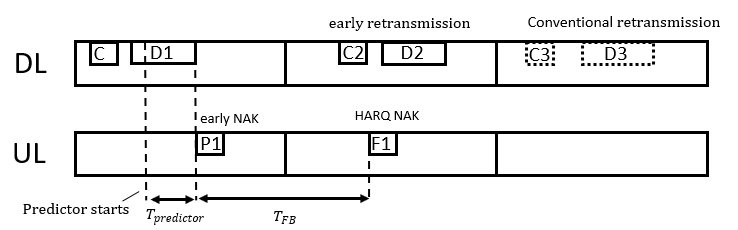
\includegraphics[scale=0.4]{fig1.png}}
\caption{Impact of $T_{FB}$ to HARQ RTT.}
\label{fig1}
\end{figure}

In an effort to optimize the HARQ feedback timing and creating more (re-)transmission opportunities within a certain latency target, a two-stage feedback is proposed. The first stage of feedback is basically a prediction about the success/failure of the transport block on PDSCH. This early prediction-based feedback is designed so that it can be transmitted by the receiver very quickly, possibly even before the complete reception of the transport block of data. It informs the transmitter about the result of the channel decoder by an intelligent estimation without passing through the whole decoding process. The second stage of feedback is a conventional HARQ feedback.

\begin{figure}[htbp]
\centerline{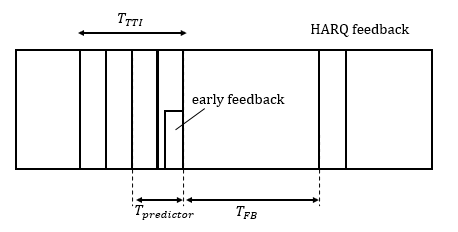
\includegraphics[scale=0.4]{fig2.png}}
\caption{Time analysis of prediction-based feedback and regular HARQ feedback.}
\label{fig2}
\end{figure}

To reduce the impact of the TTI duration in the HARQ RTT, the strategy is proposed that the receiver evaluates the error probability of PDSCH based on LLR estimation by using only a fraction of the transmitted transport block instead of using the message passing algorithm for the whole codeword as in the decoder as illustrated in Fig.~\ref{fig2}. This means that the receiver does not need to wait until the end of TTI for the complete reception of the transport block to start process (decode) the codeword, rather it can start the prediction computation just after receiving a fraction of the transport block, way before the complete reception of the transport block.

In HARQ process, time from the arrival of data in the UE to the generation of feedback is calculated by:
\begin{equation}
T = T_{TTI} + T_{FB}\label{eq4}.
\end{equation}

On the other hand, in early feedback process, time from the beginning of data transmission in the gNB to the generation of feedback in the UE is calculated by:
\begin{equation}
T' = r_{p}\times T_{TTI} + T_{predictor}\label{eq5},
\end{equation}
\begin{itemize}
    \item $r_{p}$: the ratio between the code used for prediction and the whole transmitted code
    \item $T_{predictor}$: generating early feedback time that includes the processing time of a portion of received data to predict the outcome of the whole data on PDSCH
\end{itemize}

\eqref{eq4} and \eqref{eq5} show that $T\textquotesingle$ is much smaller than $T$ when only a fraction of $T_{TTI}$ is necessary for prediction. Another reason is that $T_{predictor}$ is also smaller than $T_{FB}$ when the computation in the predictor is less complex than the decoder. Thus, early feedback can be generated before the UE receives the whole transmitted signal from the gNB and the retransmission is likely to start much earlier than the scheme with regular HARQ feedback. As a result, $T_{ReTx}$ in \eqref{eq1} decreases dramatically compared to conventional transmission scheme and latency of the system falls. 

The latency benefit in retransmission represented in the number of OFDM symbols saved by early prediction-based feedback are calculated in the following analysis. PDSCH length is 4 OFDM symbols with SCS 60kHz in Fig.~\ref{fig2}. The maximum processing time of the decoder is 0.125ms that is equivalent to 7 OFDM symbols with SCS 60kHz (1 slot with SCS 60kHz has 14 OFDM symbols spread in 0.25ms). The predictor only uses half of the transmitted bits in order to estimate the error probability of the decoder so it only uses 2 symbols and time equivalent to 2 symbols is saved. Moreover, the predictor only deals with a small portion of bits and runs few iterations of message passing algorithm in comparison to a whole codeword and full iterations of the decoder. Thereby, the predictor takes less time to provide an estimation. If the iterations of the predictor are one fifth that of the decoder (applied in simulation presented in \ref{VV}), the processing time of the predictor is 0.025ms being approximate to 2 symbols. This means that 5 symbols are saved. In total, time corresponding to 7 symbols is saved in the retransmission process and this time margin gained  might be translated  to  one more  retransmission  possibility  in the time constraint. In addition, if the UE continues to fail to decode data several times, the accumulated saving time after each NAK feedback even leads to many retransmission opportunities.  Thereby,  the reliability  requirement  of  channel  design  can  be  relaxed to  reduce  resource  utilization. 
\begin{figure}[htbp]
\centerline{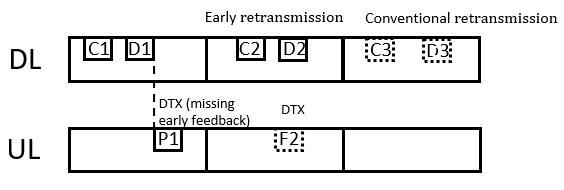
\includegraphics[scale=0.38]{fig3.png}}
\caption{Missing early feedback triggers an early transmission.}
\label{fig3}
\end{figure}

Early prediction feedback serves multiple purposes, one is to trigger an immediate retransmission when indicating the gNB about the potential PDSCH failure and secondly its absence serves to indicate a PDCCH decoding's failure. As shown in Fig.~\ref{fig3}, the gNB transmits PDCCH and PDSCH in the downlink (C1 and D1) but the UE fails to decode PDCCH so it does not know the location of PDSCH. Thereby, in this case, as it does not even know if it has been scheduled, it will send neither early prediction-based feedback nor the second stage of the classical feedback. Because there is no prediction transmitted to the gNB, it detects this discontinuous signal. Subsequently, the gNB retransmits immediately PDCCH and PDSCH (C2 and D2) instead of waiting the UE\textquotesingle s HARQ feedback (F2). The prediction even can be transmitted before the end of the initial URLLC transmission so using this strategy helps the system save much time and generates more retransmission occasions. Thus, this early prediction-based feedback will make the transmission much more robust against the PDCCH errors as an absence of prediction feedback at the gNB will be a direct indication of missed PDCCH. 

\subsection{Prediction process}\label{BB}
Early prediction-based feedback is generated by the following process. When the signal comes to the UE, after receiving a part of PDSCH codeword (a part of the TTI), the UE starts to predict the error probability of the decoding process. The rest of the codeword is still received by the UE in parallel to serve as the input of the decoder. Subsequently, the UE calculates the LLR for each bit in the predictor as
\begin{equation}
    L_{k} = log \frac{P(b_{k}=1|r_{k})}{P(b_{k}=0|r_{k})},
\end{equation}
\begin{itemize}
    \item $L_{k}$: LLR of the k\textsuperscript{th} bit in the codeword 
    \item $b_{k}$: the decoded bit of the k\textsuperscript{th} bit in the codeword
    \item $r_{k}$: the received signal of the k\textsuperscript{th} bit in the codeword
\end{itemize}

Using the base graph for LDPC code as defined in 3GPP standard \cite{b8}, the UE knows the connections among the bit nodes and the check nodes used in the predicting process so it runs the message passing algorithm in a small number of iterations to make the codeword converge to enhance the accuracy of the prediction. The predicting error probability of a bit is calculated by
\begin{equation}
    P_{e,k} = \frac{1}{1 + |L\textquotesingle_{k}|}
\end{equation}
where $L\textquotesingle_{k}$: LLR of the k\textsuperscript{th} bit after some message passing iterations.

After calculating the error probabilities of decoded bits, the UE estimates block error rate (BLER) of the whole PDSCH codeword by
\begin{equation}
   \mathrm{BLER}_{\mathrm{estimate}} = \frac{1}{M} \sum_{k} P_{e,k},
\end{equation}
where $M$ is the length of codeword used in the predictor.


From $\mathrm{BLER}_{\mathrm{estimate}}$, the UE can predict the error probability of the decoder by setting a threshold. An early ACK is generated if $\mathrm{BLER}_{\mathrm{estimate}}$ is smaller than the chosen threshold. Otherwise, an early NAK is generated. 

The prediction allows the receiver to transmit a very fast response to the transmitter regarding the success/failure of the transport block, even before receiving the full data of the transport block. This helps the gNB have more chances to retransmit the packet to boost the reliability. However, the predictor also makes the system suffer from false prediction. There are two kinds of false prediction: false negative (FN) and false positive (FP). False negative occurs when an early NAK is sent while the decoder decodes correctly the codeword. It causes a waste of resources due to the unnecessary retransmissions but it does not affect the reliability directly. False positive occurs when an early prediction ACK is sent but, in fact, the decoder fails to decode data. This means that there is no retransmission and the packet is lost. It affects the performance of URLLC transmission. Therefore, false positive is more severe than false negative. The probabilities of false negative and false positive can be adapted by changing the proper threshold in predicting ACK or NAK. The ratio between false positive and false negative is changed depending on the requirements at system level and the channel conditions.  If there is an abundance of resource as well as energy and reliability is prioritized, the system is able to accept the unnecessary retransmissions due to false negative so the threshold is adapted to make false negative happen more and vice versa when the threshold is adapted to make false positive happen more if resource needs to be shared among many UEs with strict requirements.

\subsection{Scheme to alleviate the effect of false prediction}\label{CC}

In order to avoid the harmful effects of false prediction and take full advantage of early feedback's benefits, a scheme combining both early feedback and regular HARQ feedback is proposed. The gNB is able to use HARQ feedback and then switches to early feedback when a fast retransmission is required to achieve the reliability requirement. The moment to switch from single stage classic HARQ feedback to two-stage feedback consisting of the first stage of early prediction-based feedback and the second stage of classic feedback is decided by the gNB for the sensitive URLLC traffic when it considers that latency budget is critical to meet the reliability target. When two-stage feedback is activated, the gNB has to inform the users about the activation and the resources for both stages of feedback. This activation can be sent in the higher layer signaling to the user. To keep the things simple, it would make sense to consider early prediction-based feedback similar to legacy feedback for encoding purpose at the user. Therefore, the user can apply the same encoding and transmit processing for the early prediction-based feedback as of the classical HARQ feedback.

If there are some services where dynamic control is necessary for feedback purpose or in case of sporadic traffic instants when latency budget may be very critical in some occasions, it will be advantageous to have the dynamic control over the nature of the feedback. For such cases, having an indication in the DCI for the user regarding activation of two-stage feedback will be very helpful. In one method, this indication can be a single bit flag which indicates the activation/de-activation of the two-stage feedback. The resources where UE may potentially transmit early prediction-based feedback upon activation might have been pre-assigned to the UE in the higher layer signaling.

\begin{figure}[htbp]
\centerline{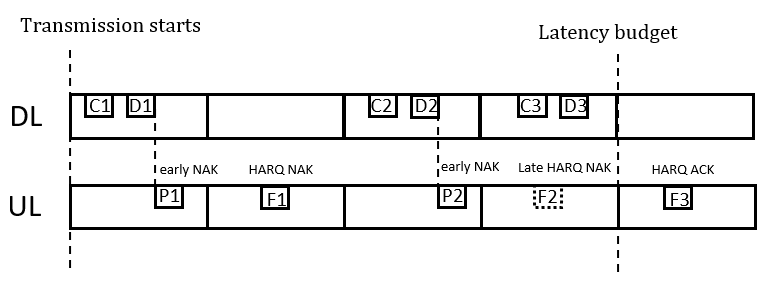
\includegraphics[scale=0.38]{fig4.png}}
\caption{Downlink transmission with early feedback and the gNB sensing latency budget.}
\label{fig4}
\end{figure}

The scheme showing the operation of downlink transmission with two-stage feedback illustrated in Fig.~\ref{fig4}. In the first transmission, the gNB sends PDCCH and PDSCH (C1 and D1, respectively) then the UE predicts a failure of the decoder and transmits an early NAK (P1) but the gNB still waits HARQ feedback (F1) to confirm that failure and retransmits the packet (C2 and D2) because it senses the remaining latency budget and recognizes that it still has enough time left to reach the target reliability with the conventional classical HARQ feedback. In the retransmission, the UE continues to predict a failure of the decoder (P2). This time, the gNB senses that latency budget is not left much and a useful retransmission is impossible in the time constraint if it waits classical HARQ feedback (F2). For this reason, in case data is actually not decoded correctly, the packet will be lost. Thus, the gNB reacts very fast to this early feedback to trigger an immediate retransmission (C3 and D3) to increase the chance that the UE can decode data correctly and the reliability of the system is boosted.

This scheme not only raises reliability of the system but also decreases the influences of false negative and especially, false positive most of the time. When latency budget still remains sufficiently, early feedback is not considered by the gNB to decide a retransmission so false prediction has no effect to the system. When latency budget is not enough for regular HARQ feedback, early feedback is used. However, in this case, false positive does not cause the detrimental effect as if early feedback is used at the beginning because the error still happens no matter early feedback is used or not because of the shortage of time to do the retransmission. Resource consumption due to false negative might happen only one time at the end of the transmission and is acceptable under the specific limit when latency and reliability are prioritized in URLLC.

\begin{figure}[htbp]
\centerline{
\includegraphics[scale=0.38]{fig5.png}}
\caption{The gNB stops a retransmission triggered by early NAK after receiving ACK HARQ feedback.}
\label{fig5}
\end{figure}

An alternative scheme is also considered when it causes the waste of resources but creates more retransmission occasion than the above scheme. If the gNB receives early ACK, it does not take that feedback into account and continues to wait for HARQ feedback in order to decide to terminate or retransmit data. Therefore, the system avoids suffering from losing packet due to false positive. On the other hand, if the gNB receives early NAK (P1) as in Fig.~\ref{fig5}, it carries out an immediate retransmission (C2 and D2). After that, if HARQ feedback is NAK, that retransmission still continues. This means that the early retransmission can be translated to more transmission occasions if data continues not to be decoded correctly. In contrast, if HARQ feedback is ACK (F1), that retransmission is no longer necessary. As illustrated in Fig.~\ref{fig5}, the gNB will stop that retransmission (C2 and D2) instantly after receiving ACK HARQ feedback to prevent from wasting resources and leave resources for other UEs. 

\section{Standardization opportunity and challenges}

Early decoding of PDSCH and the techniques to predict the outcome of PDSCH decoding are under research and will be discussed further in the ongoing release of 3GPP. The proposed scheme of two-stage feedback based on the prediction of PDSCH decoding follows this direction and can be a promising candidate to solve the latency-reliability trade-off for URLLC users and applications.

The ability of the UE must be enhanced to implement two-stage feedback when it needs a predictor for the first stage and a decoder for the second stage of regular HARQ feedback. The complexity of the UEs does not increase much when a predictor is required to be implemented because it uses the same algorithm as the decoder. The computation workload of the predictor is also not much when the predictor only deals with a portion of PDSCH. The design of the UE devices with both a predictor and a decoder should be specified to the manufacturers.  

\section{Simulation results} \label{VV}
The simulation is performed in link level to measure the reliability of prediction. LDPC code is used to encode the input PDSCH codeword with 1280 bits by base graph 2 following 3GPP standard \cite{b8}. The output codeword is modulated in QPSK and transmitted in channel. The decoder calculates LLRs and uses them to decode the receiving signal. The decoder uses min-sum message passing algorithm with maximum 25 iterations. The predictor also uses the same algorithm as the decoder but with fewer iterations that are 5.

%KHOA BEGIN
% THem ti khoang trong' duoi table, chon medskip, bigskip hoac smallskip
%\smallskip
%\smallskip
%\bigskip
\begin{table}[htbp]
\caption{Predicting error at code rate $\frac{1}{4}$}
\begin{center}
\begin{tabular}{ |p{0.5em}|p{2.5em}|p{2em}|c|c|p{2.5em}|p{2.5em}|p{3em}|}
 \hline
 \multicolumn{8}{|c|}{} \\[-1em]
 \multicolumn{8}{|c|}{\textbf{Code rate $\frac{1}{4}$}} \\
 \multicolumn{8}{|c|}{} \\[-1em]
 \hline
\textbf{\textit{$r_{p}$}} & \textbf{\textit{SNR (dB)}} &\textbf{\textit{Actual BLER}} &\textbf{\textit{FN}} &\textbf{\textit{FP}} &\textbf{\textit{Total errors}}&\textbf{\textit{T\textsubscript{saved}}}&\textbf{\textit{W\textsubscript{res}}} \\
 \hline
 \multirow{4}{1em}{\centering $\frac{1}{3}$} & $-1.4$ &$0.027$ &$0.115$ &$0.020$ &$0.135$&$0.026$&$0.112$  \\\cline{2-8}
 & $-1.35$ &$0.023$ &$0.108$ &$0.010$ &$0.118$&$0.023$&$0.106$  \\\cline{2-8}
& $-1.3$ &$0.013$ &$0.079$ &$0.012$ &$0.091$&$0.013$&$0.078$  \\\cline{2-8}
& $-1.25$ &$0.005$ &$0.058$ &$0.005$ &$0.063$&$0.005$&$0.058$  \\\cline{2-8}
 \hline
%  increase row height, number of & = number of collumn
% &&&&&\\[-1em]
 \multirow{4}{1em}{\centering $\frac{1}{2}$} & $-1.4$ &$0.035$ &$0.103$ &$0.027$ &$0.130$&$0.034$&$0.099$ \\\cline{2-8}
& $-1.35$ &$0.022$ &$0.078$ &$0.018$ &$0.096$&$0.021$&$0.076$ \\\cline{2-8}
& $-1.3$ &$0.013$ &$0.072$ &$0.013$ &$0.085$&$0.013$&$0.071$ \\\cline{2-8}
& $-1.25$ &$0.006$ &$0.053$ &$0.006$ &$0.059$&$0.006$&$0.053$ \\\cline{2-8}
 \hline
\end{tabular}
\label{tab1}
\end{center}
\end{table}

%\medskip
%KHOA END

\begin{table}[htbp]
\caption{Predicting error at code rate $\frac{1}{5}$}
\begin{center}
\begin{tabular}{ |p{0.5em}|p{2.5em}|p{2em}|c|c|p{2.5em}|p{2.5em}|p{3em}|}
 \hline
 \multicolumn{8}{|c|}{} \\[-1em]
 \multicolumn{8}{|c|}{\textbf{Code rate $\frac{1}{5}$}} \\
 \multicolumn{8}{|c|}{} \\[-1em]
 \hline
\textbf{\textit{$r_{p}$}} & \textbf{\textit{SNR (dB)}} &\textbf{\textit{Actual BLER}} &\textbf{\textit{FN}} &\textbf{\textit{FP}} &\textbf{\textit{Total errors}} &\textbf{\textit{T\textsubscript{saved}}}&\textbf{\textit{W\textsubscript{res}}} \\
 \hline
  \multirow{4}{1em}{\centering $\frac{1}{3}$} & $-2.45$ & $0.021$&$0.090 $ &$0.016 $ &$0.106$ &$0.020$ &$0.088$\\\cline{2-8}
  & $-2.4$ &$0.013$ &$0.050$ &$0.013$ &$0.063$&$0.013$ & $0.049$\\\cline{2-8}
& $-2.35$ &$0.003$  &$0.032$ &$0.002$ &$0.034$&$0.003$ &$0.032$  \\\cline{2-8}
& $-2.3$ &$0.002$ &$0.024$ &$0.001$ &$0.025$&$0.002$ & $0.024$\\\cline{2-8}
  \hline
 \multirow{4}{1em}{\centering $\frac{1}{2}$} & $-2.45$ & $0.021$&$0.086$ &$0.018$ &$0.104$&$0.020$ &$0.084$ \\\cline{2-8}
 & $-2.4$ & $0.013$&$0.041$ &$0.011$ &$0.052$&$0.013$ &$0.040$ \\\cline{2-8}
 & $-2.35$ &$0.003$ &$0.022$ &$0.002$ &$0.024$ &$0.003$ &$0.022$\\\cline{2-8}
& $-2.3$ &$0.002$ &$0.017$ &$0.002$ &$0.019$&$0.002$ &$0.017$ \\\cline{2-8}

%  increase row height, number of & = number of column
% &&&&&\\[-1em]

 \hline
\end{tabular}
\label{tab2}
\end{center}
\end{table}

Table~\ref{tab1} and Table~\ref{tab2} show the actual BLER of PDSCH, the rates of false negative, false positive and the total predicting errors (including both false negative and false positive) in a different SNR values with code rate $\frac{1}{4}$ and $\frac{1}{5}$. 

The last two columns show the probability that latency is saved (T\textsubscript{saved}) and the rate that resource is wasted (W\textsubscript{res}) defined as follows. Let's take the first case in Table~\ref{tab1} wih $r_{p}$ = $\frac{1}{3}$ and SNR = -1.4dB. Conditioned on the fact that the first transmission is a NAK, the predictor is right in 98\% of the cases and we save latency on the retransmission. A NAK happens 2.7\% of the time so we save in 2.6\% of all times (T\textsubscript{saved} = 0.026). Similarly, a ACK happens 97.3\% of the time and in that case the predictor is wrong in 11.5\% of all cases, leading to 11.2\% of all cases where we waste resources (W\textsubscript{res} = 0.112).

In each table, two cases are considered. In the first case, a half of the transmitted codeword is used to estimate the outcome. In the other case, a third of the transmitted codeword is used for prediction. The performance of the predictor in these two cases does not have a big difference so the predictor of the UE is able to use only a third of PDSCH codeword for the predicting process without influencing reliability while reducing time to generate an early feedback.

The predictor works much better with a lower rate. The reason is that at a lower rate, the codeword is longer so the portion of the codeword that is used to estimate the error probability is also longer so the sub-codeword in the predictor has a higher probability to converge.

False positive's error rate is much smaller (around 10 times smaller) than the overall prediction error. This means that false negative occurs more than false positive. However, as analyzed in \ref{BB}, false negative is less severe than false positive. Moreover, two proposed schemes in \ref{CC} also reduce the effect of false negative if they are implemented in downlink transmission when the gNB decides to use NAK prediction by sensing latency budget or stops the retransmission after receiving ACK. False positive has harmful effects but the occurring probability is very small. Besides, it also has no effect to the performance of the system in the proposed strategies. 

The two variables T\textsubscript{saved} and W\textsubscript{res} have trade-off so based on channel conditions and the requirements at system level, the threshold of the predicting algorithm in \ref{BB} can be adapted to achieve the target of latency and resource consumption. Besides, the scheme also proposes to stop transmission in case of false negative error to reduce further a waste of resources.

\section{Conclusion}

URLLC service provisioning in 5G requires an improvement in the current downlink transmission mechanism. The state-of-the-art schemes achieve reliability at the cost of latency and resource. In this paper, a downlink transmission scheme applying two-stage feedback containing an early prediction-based feedback and a HARQ feedback is presented to reduce latency of retransmission due to HARQ RTT and increase reliability of the transmission. The scheme allows flexible operating points to better achieve trade-off among latency, reliability and resource consumption as a function of system requirements and channel conditions.

\begin{thebibliography}{00}
\bibitem{ad1} H. Ji, S. Park, J. Yeo, Y. Kim, J. Lee, and B. Shim, “Ultra Reliable and Low Latency Communications in 5G Downlink: Physical Layer Aspects,”  IEEE Wireless Commun, June 2018.
\bibitem{b2} G. Berardinelli, S. Khosravirad, K. I. Pedersen, F. Frederiksen and P.Mogensen, “Enabling early HARQ feedback in 5G networks”, IEEE Vehicular Technology Conference, May 2016.
\bibitem{ad5} T-K. Le, F. Kaltenberger, U. Salim, ``Control and data channel combining for reliability enhancement in Ultra-reliable and low-latency communication's downlink transmission,'' submitted to 2019 IEEE 53rd International Conference on Communications, May 2019.
\bibitem{b1} Huawei, HiSilicon, ``PDCCH reliability for URLLC'', 3GPP R1-1719406, RAN1\#91, Reno, USA, Nov 27--Dec1, 2017.
\bibitem{b5} ZTE, Sanechips, ``Ultra-reliable part of URLLC for scheduling and HARQ procedure'', 3GPP R1-1715529, RAN1 Ad Hoc\#3, Nagoya, Japan, Sept 18--21, 2017.
\bibitem{b4} Sony, ``Reliable PDCCH operation for NR'', 3GPP R1-1716248, RAN1 Ad Hoc\#3, Nagoya, Japan, Sept 18--21, 2017.
\bibitem{b7} ZTE, ZTE Microelectronics, ``Analysis of URLLC reliability for HARQ'', 3GPP R1-1701595, RAN1\#88, Athens, Greece, Feb 13--17, 2017.
\bibitem{ad3} 3GPP TR 38.802 v14.1.0, ``Study on new radio access technology physical layer aspects.''
\bibitem{b6} 3GPP TR 38.913 v14.3.0, ``Study on scenarios and requirements for next generation access technologies.''
\bibitem{ad2} 3GPP TR 38.211 v15.0.0, ``Physical channels and modulation.''
\bibitem{b8} 3GPP TR 38.212 v15.0.0, ``Multiplexing and channel coding.''
\bibitem{ad4} Chairman's Notes RAN1 \#90, Prague, Czech Republic, Aug 21--25, 2017.

\end{thebibliography}
\vspace{12pt}


\end{document}
